\documentclass[tikz,border=10pt]{standalone}
% Scale s = 0.022663 cm/px, origin at O, y flipped
\begin{document}
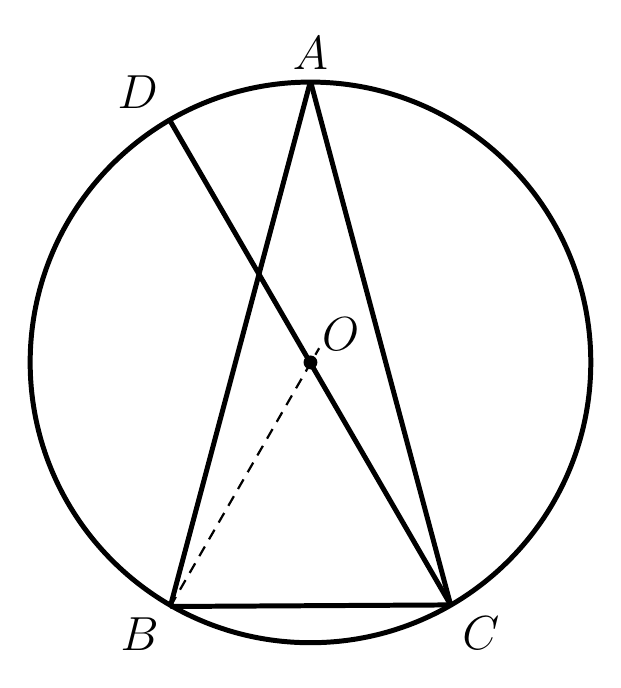
\begin{tikzpicture}[line join=round, line width=1.8pt]
  % named coordinates
  \coordinate (O) at (0,0);
  \coordinate (A) at (0,3.57);
  \coordinate (B) at (-1.78,-3.10);
  \coordinate (C) at (1.78,-3.08);
  \coordinate (D) at (-1.79,3.08);
  \coordinate (E) at (-0.65,1.14);   % unlabeled AB/CD crossing
  \coordinate (Q) at (0.11,0.18);    % dashed end, just past O toward upper right

  % circle centred at O
  \draw (O) circle[radius=3.56];

  % solid chords and diameter (BC now ends exactly at B and C)
  \draw (A) -- (B);
  \draw (A) -- (C);
  \draw (B) -- (C);
  \draw (C) -- (D);

  % dashed segment from B toward O: thinner, longer dashes
  \draw[dashed, line width=0.8pt, dash pattern=on 4pt off 3pt] (B) -- (Q);

  % centre dot
  \fill (O) circle (2.5pt);

  % labels
  \node[above, font=\fontsize{19}{22.8}\selectfont] at (A) {$A$};
  \node[above left, font=\fontsize{19}{22.8}\selectfont] at (D) {$D$};
  \node[below left, font=\fontsize{19}{22.8}\selectfont] at (B) {$B$};
  \node[below right, font=\fontsize{19}{22.8}\selectfont] at (C) {$C$};
  \node[above right, font=\fontsize{19}{22.8}\selectfont] at (O) {$O$};
\end{tikzpicture}
\end{document}